%% ============================================================
%%  代码即中间表示：用程序生成视频这一族的谱系、判据与证据强度
%%  NeurIPS 风格双栏排版（单栏标题区 + 双栏正文）
%%
%%  这是 PAPER.md 的一种渲染，不承载任何新事实。
%%  事实源是 sources/evidence/claims.csv，由 validate_research 与
%%  audit_paper 校验。本文件只负责排版。
%%
%%  编译：xelatex main.tex（两遍，交叉引用才正确）
%% ============================================================
\documentclass[10pt,twocolumn]{article}

%% 中文支持
\usepackage[UTF8,fontset=none]{ctex}

%% ---------- 标点悬挂 ----------
%% 中文双栏的行尾溢出，末字符清一色是全角右引号、右括号、逗号。
%% 原因不是可拉伸量不足，而是该行没有合法断行点：中文禁则不许标点居行首。
\usepackage{xeCJK}
\xeCJKsetup{PunctStyle=plain}

\setCJKmainfont{SimSun}[BoldFont=SimHei,ItalicFont=KaiTi]
\setCJKsansfont{SimHei}[BoldFont=SimHei,AutoFakeBold=1.2]
\setCJKmonofont{SimHei}
\setmainfont{Times New Roman}
\newfontfamily\symfont{Segoe UI Symbol}[AutoFakeBold=1.2]
\newcommand{\sym}[1]{{\symfont #1}}
\setsansfont{Arial}
\setmonofont{Consolas}

%% ---------- 版面 ----------
\usepackage[a4paper,margin=2.05cm,columnsep=0.72cm]{geometry}
\usepackage{amsmath,amssymb}
\usepackage{graphicx}
\usepackage{booktabs}
\usepackage{tabularx,array,longtable,multirow}
\usepackage{caption}
\usepackage{enumitem}
\usepackage{titlesec}
\usepackage{xcolor}
\usepackage{fancyhdr}
\usepackage[hidelinks]{hyperref}
\usepackage{xurl}

%% ---------- URL 断行 ----------
\Urlmuskip=0mu plus 1mu\relax
\makeatletter
\g@addto@macro\UrlBreaks{\do\/\do\.\do\-\do\_\do\:}
\makeatother
\newenvironment{refs}{\par\raggedright\small}{\par}

\usepackage{microtype}
\usepackage{listings}
\usepackage{placeins}
\lstset{
  basicstyle=\ttfamily\scriptsize,
  breaklines=true,
  breakatwhitespace=false,
  columns=fullflexible,
  frame=none,
  xleftmargin=0.6em,
  aboveskip=4pt,
  belowskip=4pt
}

\captionsetup{
  font=small,
  labelfont=bf,
  labelsep=quad,
  skip=4pt,
  justification=centering
}
\captionsetup[table]{position=top}

%% ---------- 中文断行规则 ----------
\XeTeXlinebreaklocale "zh"
\XeTeXlinebreakskip = 0pt plus 0.08em minus 0.02em
\XeTeXlinebreakpenalty=0

\setlength{\emergencystretch}{5em}
\tolerance=5000
\hbadness=5000
\hyphenpenalty=50
\relpenalty=50

\titleformat{\section}{\large\bfseries\sffamily}{\thesection}{0.6em}{}
\titleformat{\subsection}{\normalsize\bfseries\sffamily}{\thesubsection}{0.5em}{}
\titleformat{\subsubsection}{\normalsize\bfseries}{\thesubsubsection}{0.4em}{}
\titlespacing*{\section}{0pt}{10pt plus 2pt minus 2pt}{5pt plus 1pt}
\titlespacing*{\subsection}{0pt}{7pt plus 1pt minus 1pt}{3pt plus 1pt}
\titlespacing*{\subsubsection}{0pt}{5pt plus 1pt minus 1pt}{2pt}

\setlist[itemize]{topsep=2pt,itemsep=1pt,parsep=0pt,leftmargin=1.4em}
\setlist[enumerate]{topsep=2pt,itemsep=1pt,parsep=0pt,leftmargin=1.6em}
\newenvironment{tightlist}{\begin{itemize}\raggedright}{\end{itemize}}

\linespread{1.22}
\setlength{\parskip}{3.2pt plus 1pt}
\setlength{\parindent}{1.6em}

\pagestyle{fancy}
\fancyhf{}
\renewcommand{\headrulewidth}{0pt}
\fancyfoot[C]{\small\thepage}

\renewcommand{\topfraction}{0.92}
\renewcommand{\bottomfraction}{0.85}
\renewcommand{\textfraction}{0.08}
\renewcommand{\floatpagefraction}{0.80}
\setcounter{topnumber}{4}
\setcounter{bottomnumber}{3}
\setcounter{totalnumber}{8}

\newcommand{\textcjkc}[1]{{\CJKfamily{}#1}}

\begin{document}

%% ---------- 标题区（单栏，跨通栏） ----------
\twocolumn[{
\begin{center}
{\LARGE\bfseries\sffamily 代码即中间表示\\[2pt]
\large 用程序生成视频这一族的谱系、判据与证据强度\par}
\vspace{5pt}
{\normalsize\sffamily 18 份来源、35 条可回溯证据：五档验证信号、三类失败与三条边界\par}
\vspace{3pt}
{\small\sffamily\itshape 2026-11-18\par}
\end{center}
\vspace{6pt}
}]


\begin{quote}\small
综述 · 信息截止 2026-11-18来源 18 ｜ 证据 35 ｜ 主张 28

\end{quote}

\begin{abstract}

让 AI 生成视频，主流路线是端到端扩散模型：输入文本或图像，直接输出像素。但有一类内容它系统性做不好——精确的公式、正确的图表、规则一致的交互、与画面事件严格同步的旁白。这些内容的共同点是\textbf{存在唯一正确答案}，而像素模型只能给出「看起来像」的结果。


于是出现了另一条路线：让 agent 写一段\textbf{程序}（Manim、Blender Python、SVG/CSS、图形 DSL），由确定性渲染器把它变成视频。本文系统梳理了这条路线上的 18 项代表工作，回答三个问题：这条路线为什么成立、它现在做到什么程度、它的边界在哪。


本文的核心论断是：\textbf{代码中间表示的价值不在画质，而在于它把「视频生成」转成了三个可判定的问题——可编译、可对齐、可复现。} 这三条使验证可以自动化，从而让闭环自我改进成为可能。这正是端到端像素模型难以获得的能力。


但本文同时必须指出这条路线最尖锐的两个反证。其一，MaLiang-Harness 定义的 Program-to-Visual (P2V) gap 说明：\textbf{程序可以正确执行，却完全违背用户的视觉要求}，故「编译通过」不构成验收。其二，VibePrevisBench 观测到 \textbf{agent 会查看自己的渲染，却改不对错误}——这直接反驳了「给了视觉反馈就能自我纠正」的乐观假设。


本文据此主张：这一族当前的真实瓶颈不在生成侧，而在\textbf{「把视觉差异翻译成代码修改」}这一步。谁先解决它，谁就拿到通往更高自动化的钥匙。


\textbf{关键词}：代码生成视频；程序化动画；Manim；Blender；agentic 生成；可验证性



\end{abstract}
\section{引言}

\subsection{两类内容的根本差别}

2026 年的视频生成模型已经能产出以假乱真的画面。但把同样的问题交给它们——「画出 y = x² 与 y = 2x 的交点」、「把这个季度的营收画成柱状图」、「让角色在第三秒推开门」——结果往往不能用。原因不是画质不够，而是这类内容\textbf{有唯一正确答案}，模型无法保证对上。


VibeVideoBench 把这个观察写成了动机：Diffusion video models produce striking clips, but they cannot reliably render an exact formula, a correct chart, a rule-consistent game or narration synchronized to on-screen events{\scriptsize\texttt{[c-\hspace{0pt}why-\hspace{0pt}code]}}。四类失败对应四种确定性要求：精确的数学、精确的数据映射、确定的规则、确定的时序。


LASEV 从另一个角度说同一件事：端到端模型在要求严格逻辑与精确知识表示的场景受限{\scriptsize\texttt{[c-\hspace{0pt}why-\hspace{0pt}code]}}。它强调的是知识正确性——教学过程不能讲错。


\subsection{代码路线的主张}

代码路线的核心主张可以用 Reels-RSI 的一句话概括：A program can be read, diffed, tested and audited; pixels can only be watched{\scriptsize\texttt{[c-\hspace{0pt}auditable]}}。


这句话的分量在于它把问题从「生成质量」换成了「可审计性」。程序可以被 diff——所以「改了什么」是可追踪的；程序可以被测试——所以「对不对」是可自动判定的；程序可以被审计——所以「为什么错」是可定位的。像素做不到其中任何一件。


值得注意的是，Reels-RSI 进一步主张解释视频\textbf{本体上}就是程序：a program (script, storyboard and per-frame animation code) that a deterministic renderer turns into frames。这不只是工程选择，而是一个关于这类视频是什么的本体论判断。


\subsection{本文要回答什么}

\begin{itemize}
  \item \textbf{q1} 这一族为什么选代码而不是像素？代码中间表示带来什么能力、什么代价？
  \item \textbf{q2} 按「中间表示的类型」与「验证信号的来源」两个轴，这一族能排成怎样的谱系？
  \item \textbf{q3} 每个代表工作解决什么问题、优缺点如何？
  \item \textbf{q4} 实验结果如何比较？各种「成功率」在什么口径下成立？
  \item \textbf{q5} 这条线的天花板在哪？失败有哪些典型形态？
\end{itemize}

\subsection{主要结论}

\begin{enumerate}
  \item \textbf{代码路线的价值是可验证性，不是画质。} 程序提供可回放的真值，使「事件是否在正确时刻发生」成为可自动判定的问题，而不必依赖人评「像不像」（图 7）。
  \item \textbf{P2V gap 是这一族的核心困难。} 程序正确执行 ≠ 满足视觉要求{\scriptsize\texttt{[c-\hspace{0pt}p2v-\hspace{0pt}gap]}}。这条落差把本族的全部工作分成了两类：一类在缩小它，一类在测量它。
  \item \textbf{记忆机制的价值依模型强弱而反转。} 对强模型，规则起「审计」作用；对弱模型才是「护栏」{\scriptsize\texttt{[c-\hspace{0pt}rule-\hspace{0pt}depends]}}。这与「记忆越多越好」的直觉相反。
  \item \textbf{benchmark 已明确指出瓶颈：agent 会看但改不对。} 这不是感知问题，而是「视觉差异 \sym{→}{} 代码修改」的映射问题{\scriptsize\texttt{[c-\hspace{0pt}blind-\hspace{0pt}feedback]}}。
  \item \textbf{指标混乱是本族当前最大的可比性障碍。} 至少三种「成功率」含义不同，感知相似度与内容保真度可以差 35 个百分点{\scriptsize\texttt{[c-\hspace{0pt}look-\hspace{0pt}vs-\hspace{0pt}fact]}}。
\end{enumerate}


\section{P2V gap：这一族的核心困难}

\subsection{定义}

MaLiang-Harness 给出了本族目前最清晰的理论表述。它先陈述现象：A program can execute correctly while violating the requested{\scriptsize\texttt{[c-\hspace{0pt}p2v-\hspace{0pt}gap]}}——程序可以正确执行，却违背请求。随后定义：We introduce and define the Program-to-Visual (P2V) gap as the discrepancy between program-level correctness and visual requirement satisfaction{\scriptsize\texttt{[c-\hspace{0pt}p2v-\hspace{0pt}gap]}}。


这个定义的价值在于它一刀切开了两个此前被混为一谈的东西：「代码对不对」与「画面对不对」。前者可以用编译器与单元测试判定，后者只能渲染后判定。


\subsection{为什么这条 gap 必然存在}

根源在于\textbf{程序是意图的一种不完备编码}。同一段程序可以满足语法、通过所有 API 检查、渲染出视频，却在语义上完全不是用户想要的。MaLiang-Harness 举的例子很具体：对象出现在错误位置、动画事件发生在错误时刻。


OmniManim 把这个困难形式化为「渲染反馈感知的约束代码生成」（render-feedback-aware constrained code generation）{\scriptsize\texttt{[c-\hspace{0pt}formalization]}}——关键在于\textbf{约束只有在渲染之后才可判定}。它不是「写代码时小心一点」就能解决的问题，而是任务结构本身决定的。


\begin{figure*}[t]
\centering
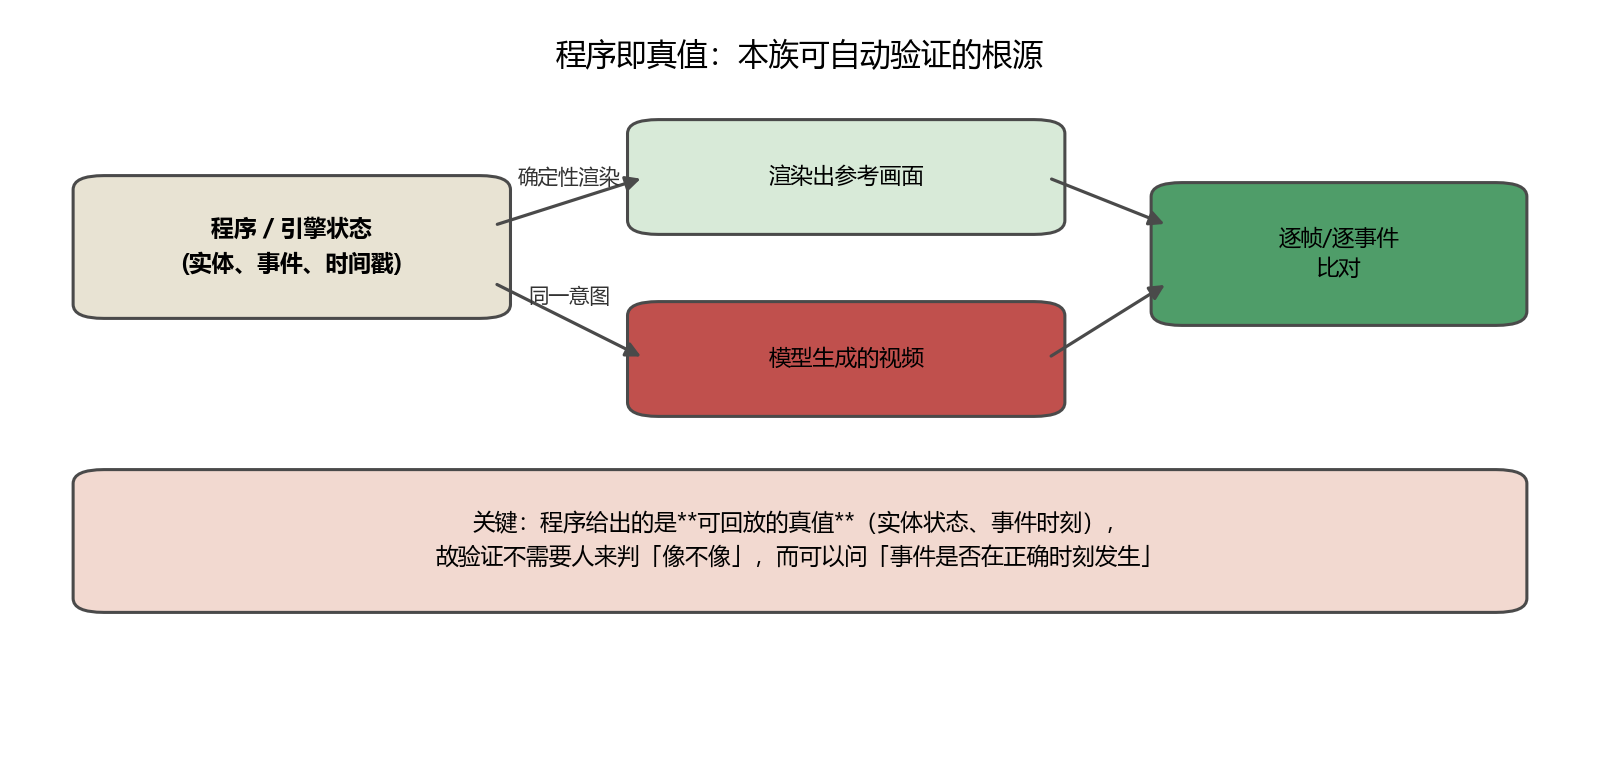
\includegraphics[width=0.86\textwidth]{../figures/fig7_framework_truth.png}
\caption{图 7　程序即真值：这是本族能自动验证的根源，也是 P2V gap 可以被量化的原因}
\label{fig:1}
\end{figure*}

\subsection{三种失败，三种信号}

本族的失败并不均质。ManiBench 给出了一个实用的二分：Syntactic Hallucinations 与 Visual-Logic Drift{\scriptsize\texttt{[c-\hspace{0pt}failure-\hspace{0pt}modes]}}。前者是引用了不存在或已废弃的 Manim API（可靠检索与版本约束修复），后者是时序错误、缺因果（只能渲染后判定）。


本文在此基础上补出第三类，因为它在本族中被反复观测到却少被单独命名：\textbf{画面像但内容错}。BVB 的结果是这一类最锋利的证据——最好模型的潜在相似度达 88.6，却只保留 53.7\% 的时空事实{\scriptsize\texttt{[c-\hspace{0pt}look-\hspace{0pt}vs-\hspace{0pt}fact]}}。


\begin{figure*}[t]
\centering
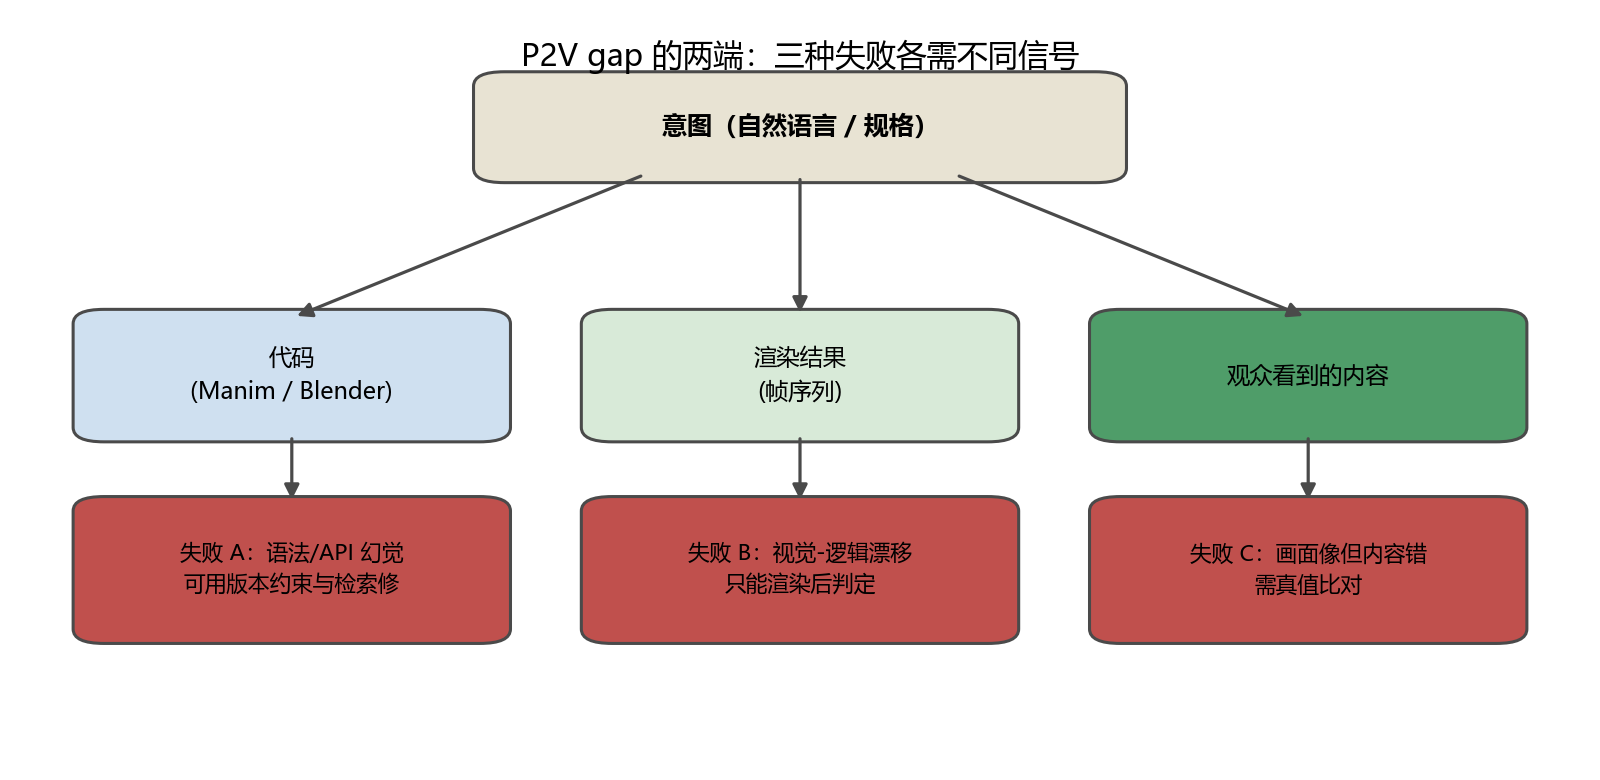
\includegraphics[width=0.86\textwidth]{../figures/fig8_framework_failure.png}
\caption{图 8　P2V gap 的两端：三种失败各需不同信号，故没有任何单一指标能覆盖全族}
\label{fig:2}
\end{figure*}


\section{谱系：中间表示 × 验证信号}

\subsection{为什么用这两个轴}

按任务分（教育、物理、Web、3D）看似整齐，却缺乏解释力：同为 Manim 教育动画，ManimTrainer 与 Reels-RSI 的机制差异远大于 ManimTrainer 与某 Blender 工作的差异。真正的分水岭在两处：\textbf{用什么中间表示}（决定可表达的时空结构）、\textbf{拿什么信号做验证}（决定能否闭环）。


\begin{figure*}[t]
\centering
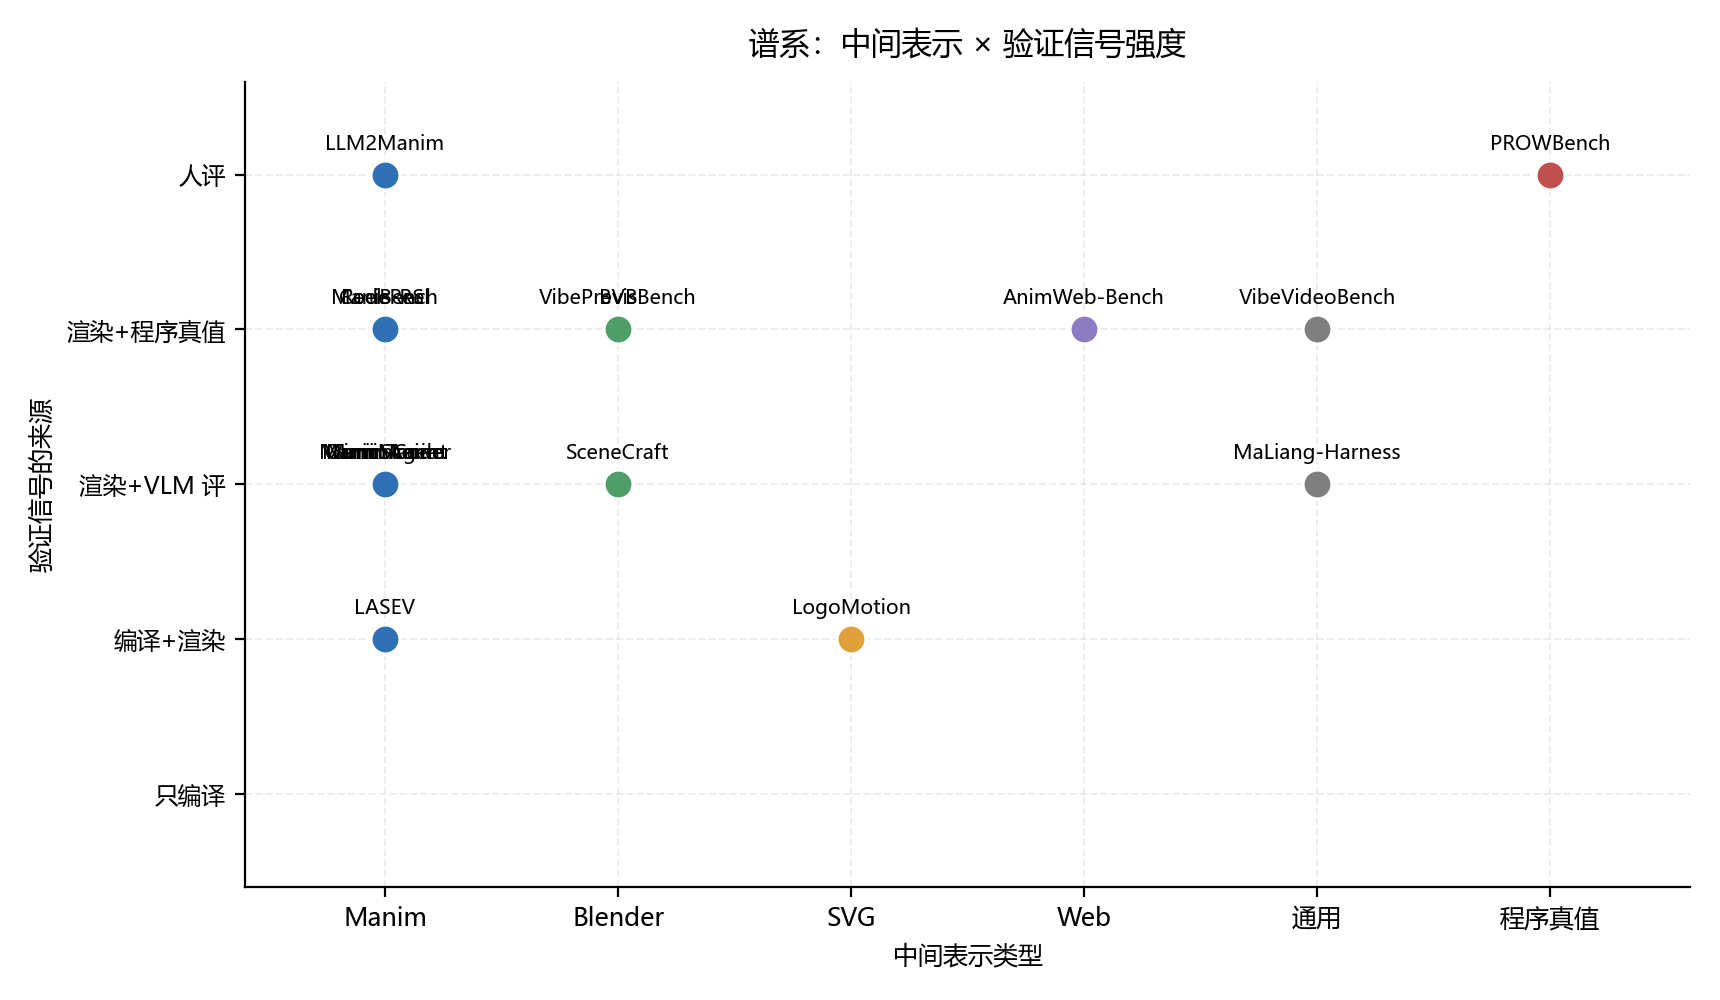
\includegraphics[width=0.86\textwidth]{../figures/fig1_lineage.png}
\caption{图 1　谱系：横轴是中间表示类型，纵轴是验证信号的来源与强度。位置越高，验证越接近「有客观真值」}
\label{fig:3}
\end{figure*}

\subsection{五档验证信号}

\begin{table*}[t]
\centering
\footnotesize
\setlength{\tabcolsep}{4pt}
\label{tab:1}
\begin{tabular}{rlll}
\toprule
档 & 验证信号 & 能判定什么 & 不能判定什么 \\
\midrule
1 & 只编译 & 语法、API 存在性 & 一切视觉与时序 \\
2 & 编译 + 渲染 & 能否渲出（RSR） & 内容是否正确 \\
3 & 渲染 + VLM 评分 & 画面是否合理 & 与规格是否严格一致 \\
4 & 渲染 + 程序真值比对 & 事件是否在正确时刻发生 & 审美与教学效果 \\
5 & 人评 & 一切 & 无法自动化，不可扩展 \\
\bottomrule
\end{tabular}
\end{table*}

这张表解释了一个常见误解：很多工作报告「94\% 渲染成功率」，读者会以为任务解决了九成。实际上 RSR 只落在第 2 档——它只表示「能渲出视频」{\scriptsize\texttt{[c-\hspace{0pt}metric-\hspace{0pt}ceiling]}}。


\subsection{全景}

\begin{table*}[t]
\centering
\footnotesize
\setlength{\tabcolsep}{4pt}
\caption{代表工作的定位。按中间表示分组，组内按验证信号强度排序}
\label{tab:2}
\begin{tabularx}{\textwidth}{llllX}
\toprule
工作 & 解决什么问题 & 中间表示 & 验证信号 & 关键机制 \\
\midrule
SceneCraft & 文本\sym{→}{}复杂 3D 场景 & Blender Python & VLM 看渲染图迭代 & 场景图先规划 + library learning \\
LogoMotion & 设计场景的 SVG 动画 & SVG / JS & 编译 + 人评 & 代码与 GUI 控件打通 \\
LLM2Manim & STEM 教学动画 & Manim & 编译 + 专家复核 & 半自动 HITL，符号台账 \\
ManimTrainer & 训练 + 推理策略对照 & Manim & 编译 + 视觉相似度 & SFT 提代码、GRPO 提视觉 \\
ManimAgent & 跨任务累积反思 & Manim & 编译 + VLM 评关键帧 & 双通道情节记忆 \\
ManimCode & 教会小模型自我纠错 & Manim & 编译 + 无参考质量反馈 & 24,034 条反馈轨迹 + 4B 模型 \\
OmniManim & 空间布局缺陷 & Manim & 渲染后结构化诊断 & 先预测关键帧布局再写码 \\
LASEV & 教学视频的严谨性 & Manim & 质量闸门 + 编译检查 & 解题/插图/旁白三 agent \\
SimuScene & 物理动画的可执行+视觉正确 & Manim & 编译 + VLM 验证问答 & 视频视觉奖励训纯文本模型 \\
Reels-RSI & 解释视频的程序级自改进 & Manim & 静态检查 + 盲评 & 规则须带 must-fail/must-pass \\
MaLiang-Harness & P2V gap & 通用 & 持久状态 + 可追溯验证 & 程序状态/历史/验证共享基准 \\
CodeReel & build 循环太慢 & Manim & 检查判决 + 精确帧复用 & 按绘制命令做帧键 \\
VibeVideoBench & 缺通用评测 & 通用 & 程序检查 + 13k 评分项 & 沙箱禁用生成模型 \\
ManiBench & API 幻觉与时序漂移 & Manim & 四档评分 & 两类失败的命名 \\
AnimWeb-Bench & Web 动画复现 & CSS/SVG & 静态保真 + 动画保真 & 124 真实网页 \\
BVB & 视频理解的正向检验 & Blender & 双 VQA + 潜在相似度 & 用程序重建视频 \\
VibePrevisBench & 4D 场景与镜头 & Blender & 规则场景 + VLM 画面检查 & 测 agent 能否改对 \\
PROWBench & 端到端模型是否忠于程序 & 程序真值 & Logic-Render 对齐 & 程序化 episode 提供真值 \\
\bottomrule
\end{tabularx}
\end{table*}


\section{Manim 线：教育动画与自我改进}

\subsection{为什么 Manim 成为主战场}

Manim 是 3Blue1Brown 为数学解释视频开发的动画库。它被这一族大量采用，原因有三：精确的数学排版（LaTeX 内嵌）、可编程的时间轴、以及庞大的公开代码语料（ManiBench 基于其 53,000 行源码与 143 个 scene 类）。


代价也很明确：Manim 的 API 面广且版本分裂（Manim CE 与 ManimGL 不兼容），这正是 ManiBench 要专门测 Version-Conflict Error Rate 的原因。


\subsection{从「一次写对」到「学会修」}

早期工作把目标定为「一次写对」。ManimTrainer 做了 17 个 30B 以下开源模型 × 9 种训练/推理策略的系统对照，最强配置（Qwen3 Coder 30B + GRPO + RITL-DOC）达 94\% 渲染成功率与 85.7\% 视觉相似度{\scriptsize\texttt{[c-\hspace{0pt}metric-\hspace{0pt}ceiling]}}。它同时给出一个重要分工：SFT generally improves code quality, while GRPO enhances visual outputs{\scriptsize\texttt{[c-\hspace{0pt}two-\hspace{0pt}ends]}}——即 P2V gap 的两端需要不同信号。


但「一次写对」的天花板很快显现。ManimCode 指出关键问题：渲染成功不代表视觉正确，且 rendering does not directly identify the code changes needed to correct these visual failures。于是它转向教模型「改」：构建 24,034 条渲染验证轨迹，保存中间程序、执行错误、视觉批评、修正动作{\scriptsize\texttt{[c-\hspace{0pt}feedback-\hspace{0pt}astrain]}}，用角色条件 SFT 训一个 4B 模型，再用 RL 训 Reviser{\scriptsize\texttt{[c-\hspace{0pt}small-\hspace{0pt}model]}}。


这一步的意义超出了性能：它把「修正能力」本身变成了可训练资产，而不是只训练「一次写对」。


\subsection{记忆：从单次反思到跨任务资产}

ManimAgent 观察到多轮反思的局限：each task remains an isolated episode: lessons learned across many reflection rounds on one task are discarded before the next begins。它的解法是双通道情节记忆——正例存成功理由、负例存已证实的坑，完全从自身任务流生长，无人工种子、不更新权重{\scriptsize\texttt{[c-\hspace{0pt}memory-\hspace{0pt}bank]}}。实测中随记忆增长，盲测人评 Pass@1 上升且反思轮数下降。


Reels-RSI 把这件事推到程序层，并加了一条本族独有的纪律：记忆必须可被单元测试。一条规则要被静态检查捕获，且必须带 must-fail 与 must-pass 两个例子才允许入库{\scriptsize\texttt{[c-\hspace{0pt}rsi-\hspace{0pt}program]}}。效果是：学到的规则抓出了规则存在之前产出的 4 个潜伏缺陷，而规则之后产出的片子里零违规。


\begin{figure*}[t]
\centering
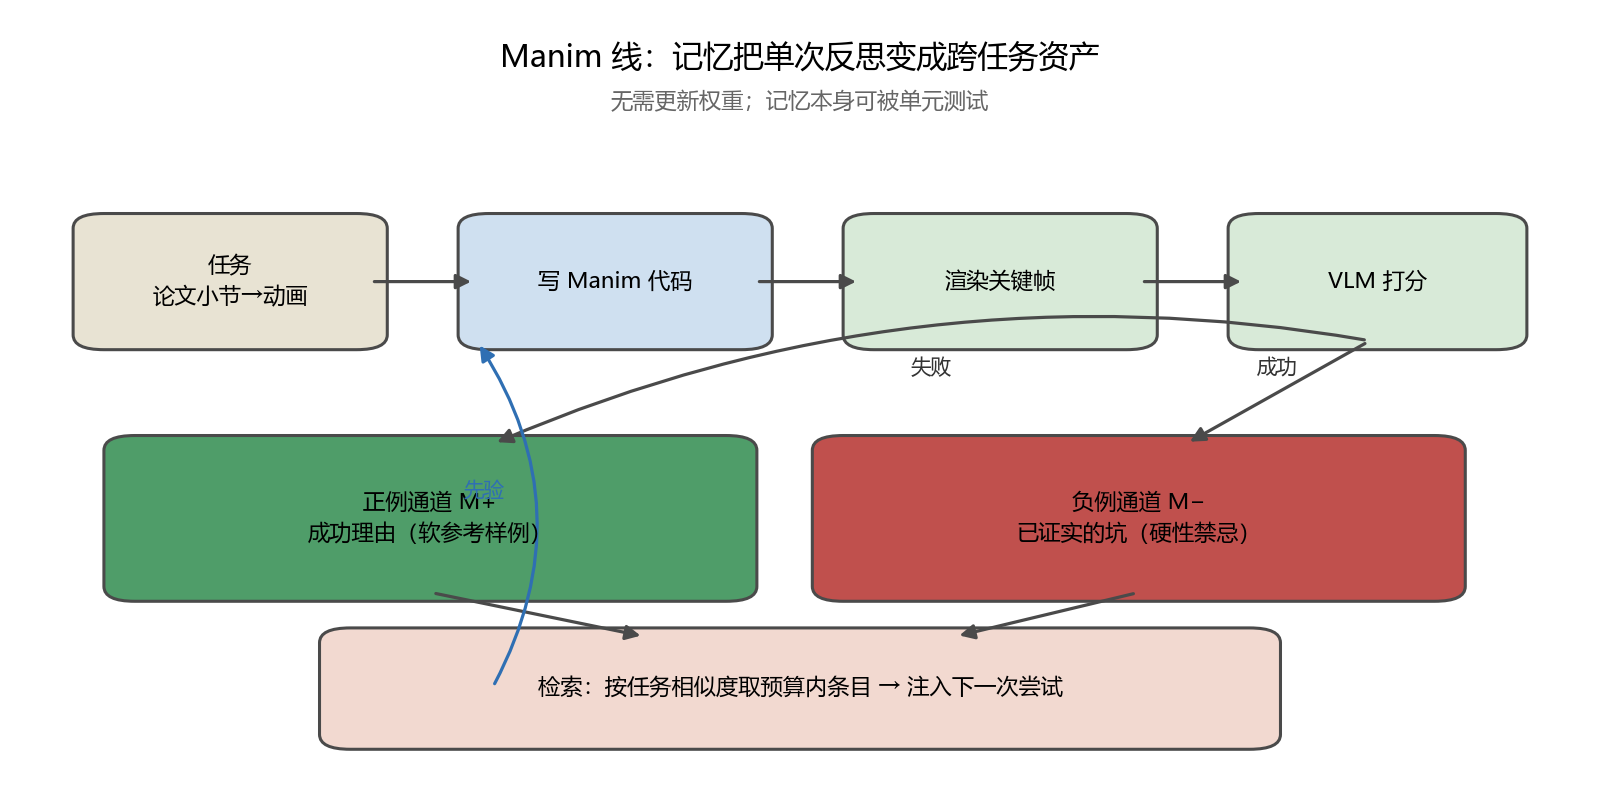
\includegraphics[width=0.86\textwidth]{../figures/fig6_framework_memory.png}
\caption{图 6　Manim 线的记忆形态。双通道记忆 + 规则入库，无需更新权重}
\label{fig:4}
\end{figure*}

\subsection{一个反向结论}

Reels-RSI 最值得注意的发现不是正面的，而是这条：that rules are an audit for a strong director (eight unguarded reels, no violation) and a guard for a weaker one (thirty violations unguarded versus five){\scriptsize\texttt{[c-\hspace{0pt}rule-\hspace{0pt}depends]}}。


也就是说，规则对强模型只起「审计」作用（它本来就不会犯），对弱模型才是「护栏」。\textbf{记忆机制的价值依模型强弱而反转}——这与「记忆越多越好」的直觉相反，也提示我们：在强模型上评估记忆机制，可能测不出任何收益。


\subsection{教学效果：唯一的实证}

LLM2Manim 是本族唯一做了教学效果实验的工作：100 名本科生 A/B 对照，动画组后测 83\% vs 幻灯片组 78\%（p<0.001）{\scriptsize\texttt{[c-\hspace{0pt}pedagogy]}}。但它同时是一条重要限制——该管线是半自动 HITL，需专家复核后才渲染。故这个效果不能归因于全自动化系统。



\section{其他中间表示：Blender、Web、SVG、通用 harness}

\subsection{Blender：空间与镜头}

Blender 路线的难点与 Manim 完全不同。Manim 主要受几何与排版约束，Blender 则要求空间推理与镜头调度。


SceneCraft 是本族早期代表作：先把场景建成场景图（含空间关系），再翻成数值约束写 Python 代码，用 VLM 看渲染图迭代；并用 library learning 把常用函数沉淀为可复用库{\scriptsize\texttt{[c-\hspace{0pt}library-\hspace{0pt}learning]}}——这是「不调权重也能累积能力」的早期形态。


VibePrevisBench 把这条线推到 4D 场景与镜头运动，并给出本族最尖锐的观测之一：给出 11 个前沿 coding agent 的轨迹分析后，它写道 agents inspect their own renders but fail to correct their errors{\scriptsize\texttt{[c-\hspace{0pt}blind-\hspace{0pt}feedback]}}。


这条观测的重要性在于它反驳了一个默认假设。很多系统的设计前提是「只要让 agent 看到渲染结果，它就能自我纠正」。VibePrevisBench 说：不，agent 确实看了，但改不对。缺的不是反馈，而是从反馈到修改的映射。


\subsection{Web 动画：时序的独立难度}

AnimWeb-Bench 把同一问题搬到 CSS/SVG 动画，得到一条更锐利的结论：reproducing webpage animations is substantially more difficult than reproducing static appearance{\scriptsize\texttt{[c-\hspace{0pt}anim-\hspace{0pt}web]}}。


这条结论的价值在于它把「有代码」与「有时序」分开了。静态外观正确不蕴含动画正确——这正是 P2V gap 在 Web 域的具体形态。同一工作还给出了正面证据：explicit frame inspection and render feedback improve the reconstruction quality{\scriptsize\texttt{[c-\hspace{0pt}render-\hspace{0pt}feedback]}}。


\subsection{通用 harness：不绑后端的框架}

MaLiang-Harness 不针对单一后端，而是提出一套通用机制：持久程序状态（PEG）、可追溯生成过程（TGP）、修订感知验证（REV），三者共享同一修订基准，使「改了什么」与「画面怎么变」被连起来。


它的定位是理论供给者——本族大部分工作都在解决具体后端的问题，只有它把 P2V gap 抽象出来。这也是本文第 2 章的主要依据。


\begin{figure*}[t]
\centering
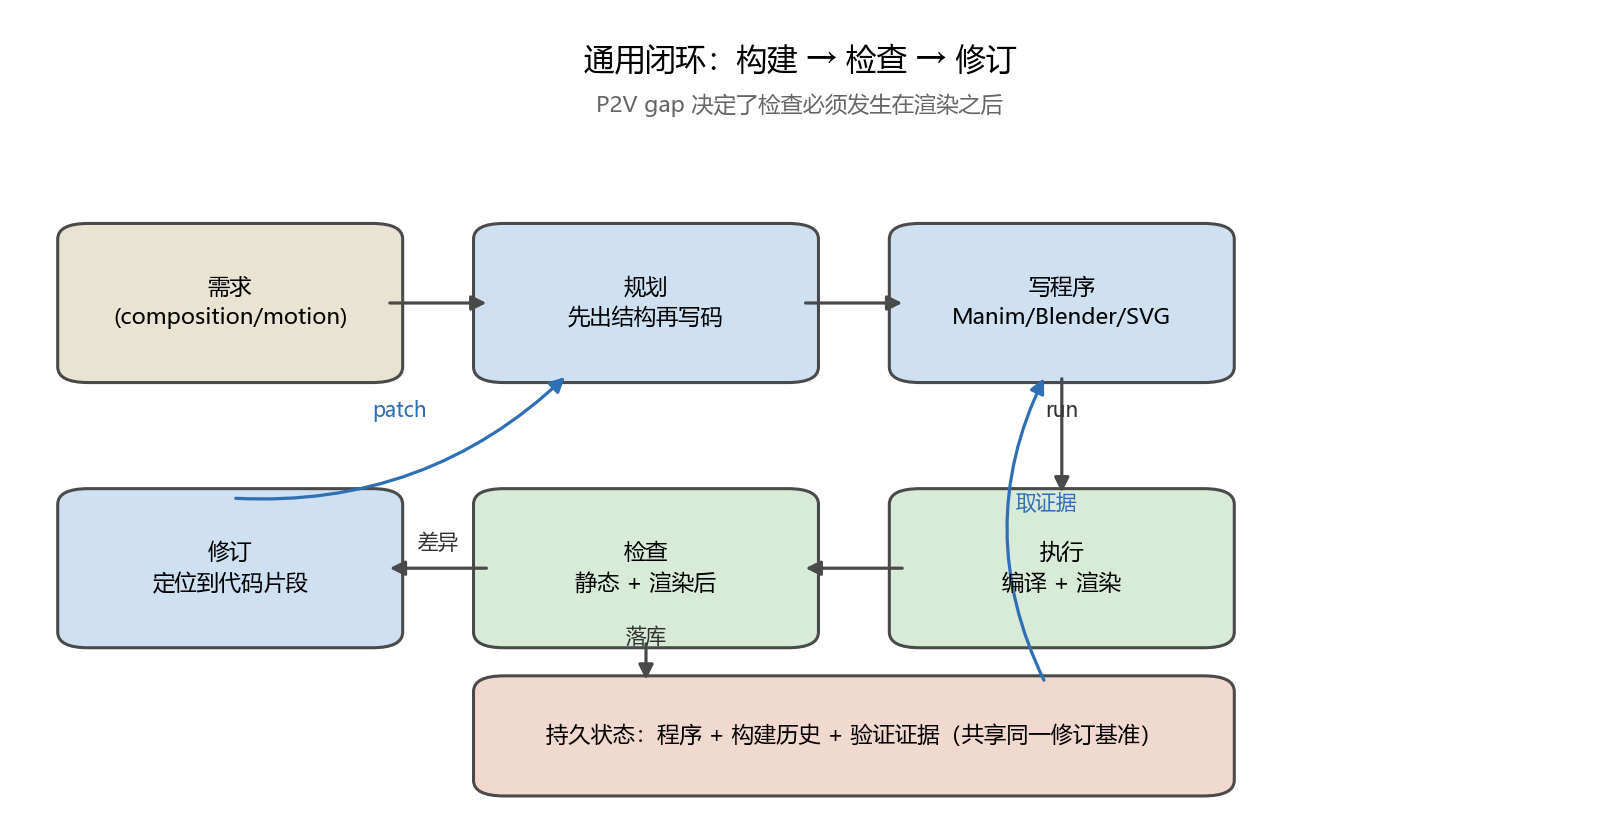
\includegraphics[width=0.86\textwidth]{../figures/fig5_framework_loop.png}
\caption{图 5　通用闭环：构建 \sym{→}{} 检查 \sym{→}{} 修订。P2V gap 决定了检查必须发生在渲染之后}
\label{fig:5}
\end{figure*}

\subsection{SVG 与可编辑性}

LogoMotion 关注一个被本族几乎所有工作忽略的维度：\textbf{交付之后怎么改}。它把代码与 GUI 编辑控件打通，使非程序员能做有目标的局部修改{\scriptsize\texttt{[c-\hspace{0pt}editability]}}。


这个视角值得单独提出，因为其余工作几乎都以「一次性交付」为目标。而在真实生产中，修改成本往往超过首次生成成本。


\subsection{一个跨后端的收敛}

把三条支线放在一起看，有一处模式重复出现在彼此独立的工作里：\textbf{先规划，再写码}。


SceneCraft 先把场景建成场景图（含空间关系），再翻译成数值约束写 Blender 代码{\scriptsize\texttt{[c-\hspace{0pt}plan-\hspace{0pt}then-\hspace{0pt}code]}}；OmniManim 先预测关键帧的布局，再写动画代码{\scriptsize\texttt{[c-\hspace{0pt}formalization]}}；LASEV 先由解题 agent 得到严格的解题步骤，再由插图 agent 写可视化代码{\scriptsize\texttt{[c-\hspace{0pt}why-\hspace{0pt}code]}}。


三者的后端完全不同（Blender / Manim / Manim），任务也不同（3D 场景 / 数学动画 / 教学视频），却收敛到同一架构。原因不难推：P2V gap 的失败大多发生在「意图到代码」的直接跳跃上，插入一个显式的中间结构（场景图、布局、解题步骤）等于给这段跳跃加了一次可检查的对齐点。



\section{基准：把「对不对」变成可计算}

\subsection{三类基准，测三种不同的东西}

本族的基准可分三类，各自测的东西不同：


\textbf{测 agent 能否写出可渲染的程序}：VibeVideoBench 是最完整的一个。它设 239 个任务、12 类、中英双语，并在沙箱内\textbf{禁用任何图像视频生成模型}，强制 agent 只能写代码{\scriptsize\texttt{[c-\hspace{0pt}vibevideo]}}。这个限制使它能真正测「代码路线」而非「模型画质」。结果是：最强系统也只在 76.3\% 的任务上满足全部核心要求。


\textbf{测端到端视频模型是否忠于程序}：PROWBench 构成这一族的\textbf{镜像}。它用程序化构造的 170 个 episode 与 600 条代理视频{\scriptsize\texttt{[c-\hspace{0pt}prowbench]}}，把实体状态与时间戳事件记成可回放的世界记录，再用两个指标检验生成的视频是否遵守规定时间轴{\scriptsize\texttt{[c-\hspace{0pt}prowbench]}}。程序在这里提供真值，被检验的是像素模型。


\textbf{测「程序重建视频」能否作为理解的判据}：BVB 把视频理解改写成「用 Blender 程序重建视频」{\scriptsize\texttt{[c-\hspace{0pt}look-\hspace{0pt}vs-\hspace{0pt}fact]}}。


\begin{figure*}[t]
\centering
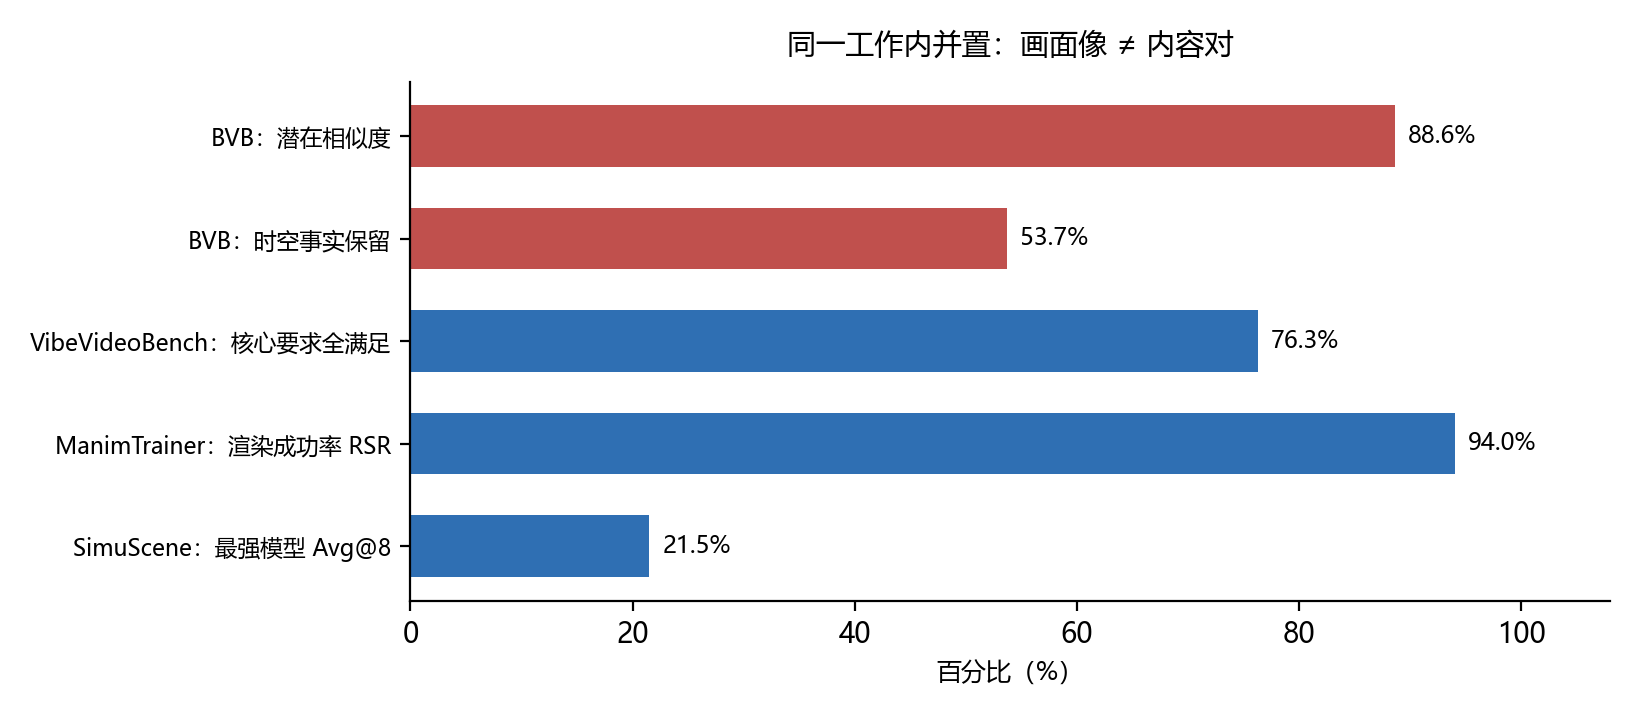
\includegraphics[width=0.86\textwidth]{../figures/fig2_gap.png}
\caption{图 2　同一工作内并置的两类指标：画面像与内容对之间的落差}
\label{fig:6}
\end{figure*}

\subsection{三个必须分开的成功率}

本族的可比性障碍主要来自指标命名混乱。至少三种「成功率」含义完全不同：


\begin{table*}[t]
\centering
\footnotesize
\setlength{\tabcolsep}{4pt}
\label{tab:3}
\begin{tabularx}{\textwidth}{llrX}
\toprule
指标 & 含义 & 典型值 & 陷阱 \\
\midrule
RSR & 能渲出视频 & 94\% & 不代表内容正确{\scriptsize\texttt{[c-\hspace{0pt}metric-\hspace{0pt}ceiling]}} \\
核心要求全满足 & 全部要求都满足 & 76.3\% & 口径严格，不可与平均分混{\scriptsize\texttt{[c-\hspace{0pt}vibevideo]}} \\
交付率 & 片子是否按时交出 & — & 缺片计 0 会改变排名{\scriptsize\texttt{[c-\hspace{0pt}metric-\hspace{0pt}sensitivity]}} \\
\bottomrule
\end{tabularx}
\end{table*}

第三行尤其容易被忽略。VibeVideoBench 发现：three quarters of the lost videos are final renders that started too late, ran too slowly or never started{\scriptsize\texttt{[c-\hspace{0pt}delivery]}}。失败发生在工程而非创作——这是一个完全独立的失败轴。


\subsection{最难的两个域}

按绝对值看，本族最难的域是物理动画。SimuScene 在 7,659 个场景上测 10 个当代模型，even the strongest model achieves only a 21.5\% Avg@8 accuracy{\scriptsize\texttt{[c-\hspace{0pt}hardest-\hspace{0pt}domain]}}。


这个数字远低于 Manim 教育动画（85.7\% 视觉相似度）与 Web 动画。原因不难理解：物理动画要求「画面的动态」必须符合物理定律，而不只是几何排布正确——这比 P2V gap 又多了一层领域知识约束。



\section{优点与局限的横向对照}

把各工作的优缺点并置，能看出一件在单篇论文里看不到的事：\textbf{优点几乎都来自「把验证做得更接近客观真值」，局限几乎都来自「验证信号仍依赖人的判断」}。


\begin{table*}[t]
\centering
\footnotesize
\setlength{\tabcolsep}{4pt}
\caption{优点与局限的横向对照。缺点一列全部来自各工作的自陈 limitations 或基准实测}
\label{tab:4}
\begin{tabularx}{\textwidth}{lXl}
\toprule
工作 & 优点 & 缺点 \\
\midrule
SceneCraft & 场景图先规划；library learning 可累积 & 只到静态场景与短镜头；无时序正确性指标 \\
LogoMotion & 唯一重视可编辑性与局部修改 & 面向设计 logo，不涉长视频与叙事 \\
LLM2Manim & 唯一有教学效果实验（100 人 A/B） & 半自动、需专家复核，不能归功于自动化 \\
ManimTrainer & 17 模型 × 9 策略的系统对照 & 94\% RSR 只表示能渲出，不代表内容对 \\
ManimAgent & 记忆完全自生长，无需人工种子 & 评测是固定探针，未验证跨领域迁移 \\
ManimCode & 反馈轨迹成为可训练资产；4B 可用 & 依赖渲染验证的规模，冷启动成本高 \\
OmniManim & 把约束形式化为渲染后才可判 & 布局预测本身会引入新的失败模式 \\
LASEV & 动机论证最清晰（逻辑严谨性） & 三 agent 编排成本高；无开源复现 \\
SimuScene & 物理域最扎实的数据与人工核验 & 21.5\% Avg@8 说明远未可用 \\
Reels-RSI & 规则可单元测试；能审计历史产物 & 对强模型价值有限，收益依赖模型弱 \\
MaLiang-Harness & P2V gap 的定义最清晰 & 通用框架，未针对具体后端优化 \\
CodeReel & 不牺牲质量即可提速 & 只优化执行层，不改善生成内容 \\
VibeVideoBench & 唯一通用且禁用生成模型的基准 & 排名对交付口径敏感 \\
ManiBench & 把失败类型学讲清楚 & 150-\hspace{0pt}200 题规模偏小；仅 Manim \\
AnimWeb-Bench & 揭示「动画远比静态难」 & 仅 Web 域；需参考视频与静态资产 \\
BVB & 把理解任务转成可验证的程序重建 & 88.6 vs 53.7 的落差说明指标仍偏感知 \\
VibePrevisBench & 揭示 agent 会看但改不对 & 需 Blender 与灰模渲染，复现门槛高 \\
PROWBench & 程序真值使验证可自动化 & 只测端到端模型，不测代码 agent \\
\bottomrule
\end{tabularx}
\end{table*}


\section{被忽略的一条轴：成本}

本族几乎所有工作都以质量为唯一目标，但 CodeReel 量化了另一条轴：一部完成片的中位数是 10 次 build、\$2.85 模型调用、11 分钟{\scriptsize\texttt{[c-\hspace{0pt}build-\hspace{0pt}cost]}}；其中 37.5\% 的帧是重复渲染{\scriptsize\texttt{[c-\hspace{0pt}build-\hspace{0pt}cost]}}。


它的优化不改变生成内容，只改执行层：按绘制命令给帧做键做精确复用，检查先行、渲染并行，把等待时间降 36.3\%（对 Rebuild）与 57.9\%（对 Sequential）{\scriptsize\texttt{[c-\hspace{0pt}codereel]}}。


这里必须强调口径纪律：这两个数字基线不同，不可混用，更不可与质量类指标相减。


\begin{figure*}[t]
\centering
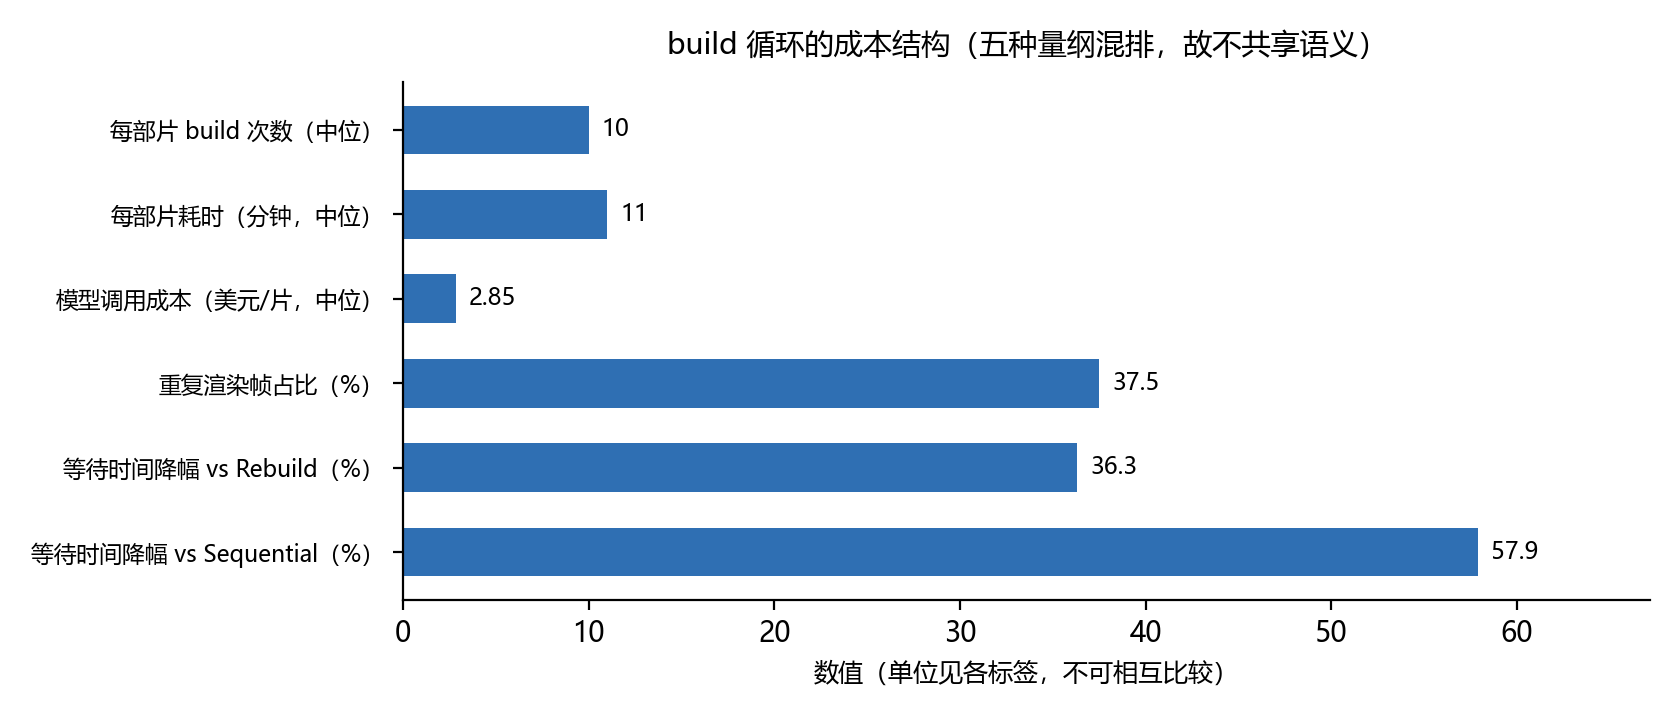
\includegraphics[width=0.86\textwidth]{../figures/fig4_cost.png}
\caption{图 4　build 循环的成本结构。五项量纲不同，仅作数量级展示，不可相互比较}
\label{fig:7}
\end{figure*}

\begin{figure*}[t]
\centering
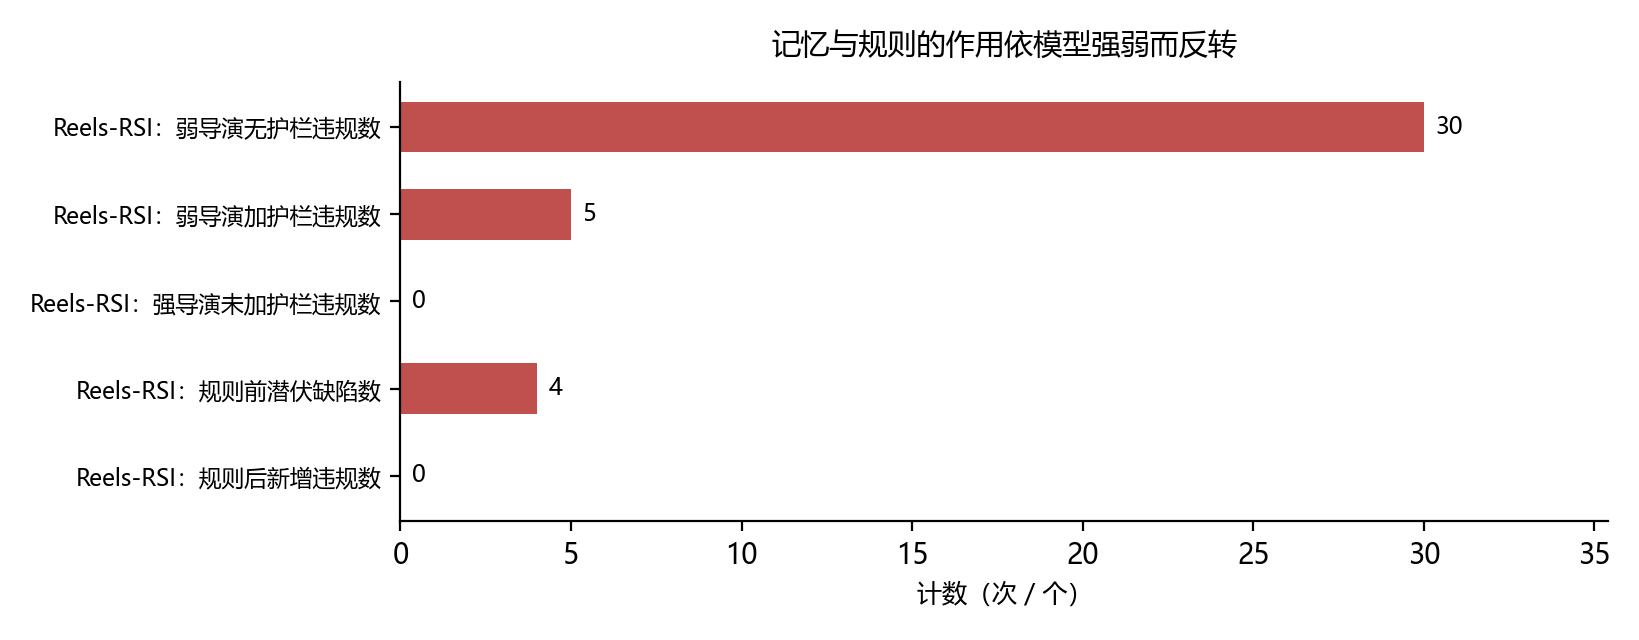
\includegraphics[width=0.86\textwidth]{../figures/fig3_memory.png}
\caption{图 3　记忆与规则的作用依模型强弱而反转}
\label{fig:8}
\end{figure*}


\section{边界与未解问题}

\subsection{三条边界}

\textbf{边界一：验证信号的上限是「程序真值」。} 第 3.2 节的五档里，只有第 4 档（渲染 + 程序真值比对）能同时做到自动化与客观。但这一档只在程序本身能提供真值时可用——教育动画的「讲得对不对」、审美、教学效果都不行，仍需第 5 档人评。


\textbf{边界二：P2V gap 的缩小依赖「视觉差异 \sym{→}{} 代码修改」的映射。} VibePrevisBench 的观测说明这一步尚未打通{\scriptsize\texttt{[c-\hspace{0pt}blind-\hspace{0pt}feedback]}}。目前的替代方案是加大模型规模或加长反思轮数，但两者都不解决映射本身。


\textbf{边界三：领域知识的视觉化是另一层困难。} 物理动画的 21.5\% 说明即使代码正确、几何正确，仍可能因为不符合物理定律而失败{\scriptsize\texttt{[c-\hspace{0pt}hardest-\hspace{0pt}domain]}}。这一层不在 P2V gap 的表述范围内。


\subsection{本文最想强调的一条}

如果把这一族的所有发现压缩成一句，本文认为应是：\textbf{「给了反馈」与「能用上反馈」是两件事。}


支持这一判断的证据来自两侧。正面：显式看帧与渲染反馈确实提升质量{\scriptsize\texttt{[c-\hspace{0pt}render-\hspace{0pt}feedback]}}，用代码生成视频的视觉奖励确实能训练出更好的模型{\scriptsize\texttt{[c-\hspace{0pt}render-\hspace{0pt}as-\hspace{0pt}reward]}}。反面：agent 会看自己的渲染却改不对{\scriptsize\texttt{[c-\hspace{0pt}blind-\hspace{0pt}feedback]}}。


两者并不矛盾——问题不在反馈的有无，而在反馈到动作之间的那一步是否被显式建模。Reels-RSI 的规则库、ManimCode 的修正轨迹、MaLiang-Harness 的 TGP，都是对这一步的不同尝试。


\subsection{未解问题}

\begin{enumerate}
  \item \textbf{如何自动构造验证器？} 目前大多数验证靠人写规则或人评。若验证器本身能成为被改进的对象，这一族才可能真正闭环。
  \item \textbf{跨域迁移的边界在哪？} Manim 上的记忆能否迁到 Blender？目前无工作回答。
  \item \textbf{交付工程能否标准化？} 四分之三的失败在交付，但几乎没有工作把交付当作研究对象（CodeReel 是例外）。
  \item \textbf{审美与教学效果如何自动化？} 这是第 5 档人评覆盖的部分，也是最难自动化的部分。
\end{enumerate}


\section{结论}

本文梳理了「用代码作为中间表示生成视频」这一族的 18 项代表工作。核心结论有三。


\textbf{第一，这条路线成立的理由是可验证性，而非画质。} 程序提供可回放的真值，使「事件是否在正确时刻发生」成为可自动判定的问题。这是端到端像素模型难以复制的通路，也是本族能发展出闭环自我改进的前提。


\textbf{第二，P2V gap 是全族的组织性困难。} 程序正确执行不等于满足视觉要求。这条 gap 把工作分成两类：缩小它的（记忆、规则、布局先验、修订机制）与测量它的（各基准）。两类都必要，但目前还没有一类能宣称解决了它。


\textbf{第三，瓶颈在「视觉差异 \sym{→}{} 代码修改」的映射。} agent 会看但改不对，这一观测把问题定位得非常具体。谁先解决它，谁就拿到通往更高自动化的钥匙。


最后需要坦白本文的局限：本族工作高度分散在不同社区（教育技术、图形学、agent 系统），检索极可能仍有遗漏；且多数工作的实验口径不同，本文虽然逐项标注了判据，但跨工作的定量比较仍不成立。



\section{参考文献}

本文证据全部来自 \texttt{sources.csv} 记录的 18 个来源，逐条引文可在 \texttt{evidence.csv} 核对（E1 不变量保证每条 quote 是快照的逐字子串）。


\begin{enumerate}
  \item VibeVideoBench: Evaluating Multimodal Agents on Code-Driven Video Generation. arXiv:2610.35864, 2026-10-26.
  \item PROWBench: Do Video Models Render What the Program Specifies? arXiv:2610.02205, 2026-10-01.
  \item ManiBench: A Benchmark for Testing Visual-Logic Drift and Syntactic Hallucinations in Manim Code Generation. arXiv:2603.13251, 2026-02-24.
  \item AnimWeb-Bench: Benchmarking Animated Webpage Code Generation from Videos. arXiv:2611.09769, 2026-11-06.
  \item VibePrevisBench: Evaluating Agentic Coding for 4D Scene Generation in Blender. arXiv:2611.15789, 2026-11-11.
  \item BVB: Benchmarking Agentic Video Understanding via Programmatic Reconstruction in Blender. arXiv:2609.15478, 2026-09-14.
  \item Reels-RSI: Program-Level Self-Improvement for Code-Rendered Explainer Videos. arXiv:2610.14495, 2026-10-10.
  \item ManimAgent: Self-Evolving Multimodal Agents for Visual Education. arXiv:2606.30296, 2026-06-29.
  \item ManimCode: Learning Visual Self-Correction for Educational Animation. arXiv:2611.08294, 2026-11-05.
  \item See Before You Code: Learning Visual Priors for Spatially Aware Educational Animation Generation. arXiv:2605.15585, 2026-05-15.
  \item Training and Agentic Inference Strategies for LLM-based Manim Animation Generation. arXiv:2604.18364, 2026-04-20.
  \item LLM2Manim: Pedagogy-Aware AI Generation of STEM Animations. arXiv:2604.05266, 2026-04-07.
  \item Beyond End-to-End Video Models: An LLM-Based Multi-Agent System for Educational Video Generation. arXiv:2602.11790, 2026-02-12.
  \item Training and Benchmarking Code Generation for Physics-Inspired Animations. arXiv:2602.10840, 2026-02-11.
  \item CodeReel: Accelerating Code-to-Video Agents with Exact Frame Reuse and Blocking-Aware Scheduling. arXiv:2611.22967, 2026-11-17.
  \item SceneCraft: An LLM Agent for Synthesizing 3D Scene as Blender Code. arXiv:2403.01248, 2024-03-02.
  \item MaLiang-Harness: A Programmable Path to Image and Video Generation. arXiv:2609.34309, 2026-09-28.
  \item LogoMotion: Visually-Grounded Code Synthesis for Creating and Editing Animation. arXiv:2405.07065, 2024-02-24.
\end{enumerate}


\section{附录 A　研究方法与可复现性}

归档位于 \texttt{research/code-to-video/}，包含 brief、检索、来源登记、证据生成、论文数据与图。


三条机器校验的不变量必须通过：


\begin{itemize}
  \item \textbf{E1} 每条 quote 是快照的逐字子串
  \item \textbf{S1} 每条来源的 fetched\_at 带时区
  \item \textbf{D1} 同一 document 不得有两个 content\_hash
  \item \textbf{C1} confidence=high 需至少一条 trust\_tier=primary 的 supports 证据
\end{itemize}

当前状态：18 来源、35 证据、28 主张（全部 high）、E1 可校验 35/35、C1 违反 0。



%% 参考文献已由 body.tex 从 PAPER.md 的「参考文献」章生成，
%% 故不再 %% 参考文献。逐条对应 sources.csv 的 18 个来源。
%% arXiv 链接用 \url 并依赖 main.tex 的 xurl + \UrlBreaks 设置才能断行，
%% 否则长 token 会把同段中文逐词拆行。
\begin{refs}
\section*{参考文献}
\small

\begin{enumerate}[label={[\arabic*]},leftmargin=2.1em,itemsep=1pt,topsep=2pt]

\item VibeVideoBench: Evaluating Multimodal Agents on Code-Driven Video Generation.
  arXiv:2610.35864, 2026.

\item PROWBench: Do Video Models Render What the Program Specifies?
  arXiv:2610.02205, 2026.

\item ManiBench: A Benchmark for Testing Visual-Logic Drift and Syntactic
  Hallucinations in Manim Code Generation. arXiv:2603.13251, 2026.

\item AnimWeb-Bench: Benchmarking Animated Webpage Code Generation from Videos.
  arXiv:2611.09769, 2026.

\item VibePrevisBench: Evaluating Agentic Coding for 4D Scene Generation in Blender.
  arXiv:2611.15789, 2026.

\item BVB: Benchmarking Agentic Video Understanding via Programmatic Reconstruction
  in Blender. arXiv:2609.15478, 2026.

\item Reels-RSI: Program-Level Self-Improvement for Code-Rendered Explainer Videos.
  arXiv:2610.14495, 2026.

\item ManimAgent: Self-Evolving Multimodal Agents for Visual Education.
  arXiv:2606.30296, 2026.

\item ManimCode: Learning Visual Self-Correction for Educational Animation.
  arXiv:2611.08294, 2026.

\item See Before You Code: Learning Visual Priors for Spatially Aware Educational
  Animation Generation. arXiv:2605.15585, 2026.

\item Training and Agentic Inference Strategies for LLM-based Manim Animation
  Generation. arXiv:2604.18364, 2026.

\item LLM2Manim: Pedagogy-Aware AI Generation of STEM Animations.
  arXiv:2604.05266, 2026.

\item Beyond End-to-End Video Models: An LLM-Based Multi-Agent System for
  Educational Video Generation. arXiv:2602.11790, 2026.

\item Training and Benchmarking Code Generation for Physics-Inspired Animations.
  arXiv:2602.10840, 2026.

\item CodeReel: Accelerating Code-to-Video Agents with Exact Frame Reuse and
  Blocking-Aware Scheduling. arXiv:2611.22967, 2026.

\item SceneCraft: An LLM Agent for Synthesizing 3D Scene as Blender Code.
  arXiv:2403.01248, 2024.

\item MaLiang-Harness: A Programmable Path to Image and Video Generation.
  arXiv:2609.34309, 2026.

\item LogoMotion: Visually-Grounded Code Synthesis for Creating and Editing
  Animation. arXiv:2405.07065, 2024.

\end{enumerate}
\end{refs}
——那会排出两份重复的文献表。
%% references.tex 保留在目录里仅作人工校对用。

\end{document}
